% Modified 

\documentclass{l3proj}

\usepackage{url}

\begin{document}
\title{Team H: Mind Game}
\author{Jarana Manotumruksa\\
	Craig Martin \\
	David McKenna \\
	Rafael Nunes \\
	Demian Till \\
	}
\maketitle
\begin{abstract}

The abstract goes here

\end{abstract}
\educationalconsent
\tableofcontents
%==============================================================================
\chapter{Introduction}
\label{intro}
% To be updated

	The reader of this report is expected to be familiar with terms and concepts related to
general computer science but not necessarily artificial intelligence. The reader is also
expected to be familiar with the game of chess.

	Mind games are games in which there is no element of luck. The outcome of every action
can be precisely calculated allowing, in theory, a player with enough time on their hands to
play perfectly. In other words, such a game can be ‘solved’ in theory.

	Of the many popular mind games, we thought that chess would best fit our purposes.
Playing a game of chess is complicated enough a problem to be well beyond being solved
by any foreseeable computer. This means that subtler techniques need to be employed in
order to create an AI that can play effectively such as estimating the value of different
positions that could occur in the future and using these estimates to narrow down which of
the available moves should be considered further when taking a turn. This provides
interesting programming and intellectual challenges.

	Another point in favour of chess is that the rules are complicated enough to provide further
programming challenges. There are many different pieces, each with different ways of
moving and capturing. Additionally, some moves rely on what has happened previously in
the game such as castling which relies on the king and the rook never having moved, and
\emph{en passant} which is available only for a single turn after a particular event has occurred.
Also, checking for stalemate requires comparing previous positions for repetition.

	Finally, chess was the only mind game fulfilling the above criteria with which every
member of the team was familiar. It is also one of the most popular games in the world,
which will make it all the more satisfying to build an AI for.

	Unlike some of the other projects, a huge amount of work has already been done on the
particular problem of writing chess AIs. With our very limited resources, we had
absolutely no chance of bettering the top existing projects in any way. This means that we have rather modest aims
relative to the current state of the art.

	Following requirements gathering and discussion with the project supervisor, we aimed, at the minimum, to build a chess AI that can consistently beat a novice player, obeying and accounting for all rules of the game with the possible exceptions of
\emph{en passant} and stalemate, along with a functional UI displaying the state of the game and
allowing the player to make moves. Another requirement would be that the AI would need to guarantee making moves within
a short time frame, say, 0 – 20 seconds on a typical home computer.

	Ultimately, we aimed to make an AI capable of beating a fairly skilled player,
acknowledging the full rule set, providing many more UI features such as displaying legal
moves, displaying previously played moves, allowing the user to undo moves and saving
and loading games. We would also like to offer multiple difficulty levels/playing styles and
enable the AI to play effectively to a clock, aborting the search before time runs out and
playing the best move according to the most accurate estimates made so far.

	The extensive past work on the subject offers a rich pool of knowledge to guide our efforts. We could draw back on many features of previously implemented chess engines such as;the mini-max search algorithm, alphabeta pruning, quiescence, various forms of board representation and ways of representing pieces. However, a challenge lies in selecting the most appropriate of these for our project

	The rest of the dissertation will detail the process and results of requirements gathering,
and then go on to explain the final design of our program, the process that lead to it and the dissertation will discuss how well the aims of the project were realised, and what could be improved.

\section{Basic Computer Chess Components} 

	Firstly, this dissertation will introduce and explain basic computer chess components that were used or considered in the making of this project. 

\subsection{Piece and Board Representation}

	One of the first problems that must be considered when designing a chess engine is how the board and the pieces will be represented in memory. A well-implemented board representation aids the system not just in ease of programming, but also overall performance. Ideally, the implementation will aid the programmer in locating pieces, identifying the colour and type of pieces, move generation, and checking for illegal moves. A poor implementation will result in more design issues later, as finding pieces and move generation become difficult and require large amounts of manual hard-coded checking to be done, which in turn results in a large performance drop. As such, it is important to consider the representation that will be chosen in the engine.

\subsubsection{Board Representation}

	Many factors have to be considered when designing the chess engine's board storage. Originally, it was beneficial to use the smallest possible data structure, as memory space was small and efficient usage of the limited space was necessary. Since memory space is no longer the issue it used to be, modern chess engines aim for speed, efficiency and ease of use with regards to move generation, checking for illegal moves etc. Boards must also store other information about the game, such as the time until stalemate and eligibility to castle, but these can be stored as simple boolean objects with little difficulty compared to the structure of the board itself. Numerous data structures have been developed to represent boards in memory.


	The simplest representation of a board is a single 64 element array, with each square being numbered horizontally from one corner of the board. This uses up the least amount of space, and initially appears to make moving a piece simple: By simply changing the index of a piece by a number that the piece is legally allowed to move by, the new location can be determined. An alternate form uses a two dimensional 8x8 array, which presents a simple mapping of rank and file as shown in a real chess board with a minimal increase in complexity for determining movement. 


	However, problems arise when trying to determine illegal moves that take place off the edge of the board. As long as a piece can move unopposed by other pieces, it can travel through one side of the board and emerge on the next or previous rank of the other side. For example, a rook at h4, the far right of the board, could travel right and emerge on a5. Assuming  that it did not encounter any other pieces, the rook could travel anywhere on the board by moving horizontally. Dealing with this problem results in a massive decrease in performance as every instance of this possibility must be checked to ensure that a piece cannot move off the board. As shown by the example below: \\

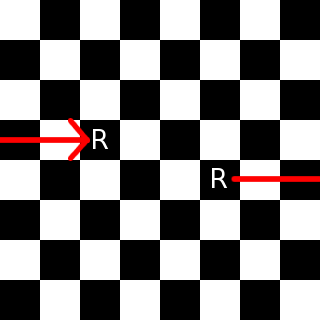
\includegraphics[scale = 0.75]{images/illegalmove.png}

	A solution to this problem is to enlarge the array used to store the board to include border spaces, which signify the edge of the board. Typically, two border squares are used at the ends of each file, and one on both sides of each rank. These squares contain a value to signify the end of the board, and as such any piece that moves on them is committing an illegal move. Two squares are necessary for the border as the knight is a stepping piece and as such can move two squares without passing through the first; only one border square is necessary on each side as any two-square stepping move will wrap around onto the border square on the other side. This eliminates the issue with checking illegal moves with only a small increase in memory space required.

	Another method used to represent boards is the 0x88 method, which uses the shape of the board and properties of hexadecimal numbers to determine illegal moves. The data structure used is an array of 128 elements, which is arranged as two identical chess boards side by side, with the numbering continuing horizontally across both boards before wrapping around to the next rank. This is shown in the diagram below:\\

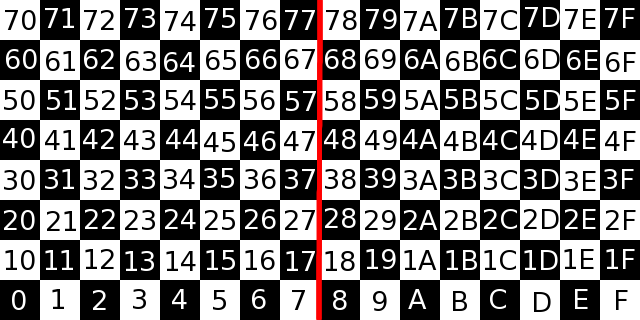
\includegraphics[scale = 0.5]{images/0x88.png}

 	The left board is used to contain the legal squares, while the right contains illegal ones; since two boards side by side produce 16 squares for each rank, certain hexadecimal properties hold with regards to the index of each square. When performing a bitwise and operation with the hexadecimal number 0x88 (10001000), any square on the right side of the board will result in a non-zero value, while every square on the left will result in zero. In this way, every illegal move can be determined with the same simple check. The 0x88 method is more efficient than the border-controlled data structure, as there is no need to initialise the board with the illegal value.

	The bitboard technique uses a number of 64-bit words to represent different aspects of the board, with each square containing a single bit to represent its state with regard to that aspect. For example, one word may contain the location of white pawns, while another will contain the position of one side's rooks. This allows the engine to take advantage of quick bitwise operations for each aspect of the board,  and stores a large amount of data in a very small format.

\subsubsection{Piece representation}

	Having decided on a particular data structure for the board used by the engine, it is now necessary to choose a representation for pieces in the game. Again, the simplest option would be to represent each piece as an integer. Each number would represent a different kind of piece, with positive and negative numbers used to differentiate colour.

	Immediately, several issues arise with this choice. The piece cannot know its own rules for movement, being simply a number. Movement must be checked when the piece tries to move in a lengthy and unwieldy test. In addition, it is difficult to find the location of all of one side’s pieces; a search of the whole board must be carried out.

	It is more efficient to introduce a separate structure to represent pieces on the board. Ideally, the location and type of all pieces for one colour can be used, cutting down the search time required to find a specific piece. In addition, a piece can store its own movement information, making the process of move generation and checking for illegal moves more streamlined.

\subsection{Artificial Intelligence}

	The development of a chess artificial intelligence requires multiple components to be working together to produce a quick, clever response to any board layout. A balance must be struck between speed and performance, for a complex evaluator will produce a good move but will spend unmanageable amounts of time doing so.

\subsubsection{Move generation}

	The first step in the artificial intelligence evaluation process for each move made by the AI is the generation of all available moves from the current board position. The representation of the board and pieces helps greatly in this task, as each available piece must be checked to find all moves it can make that are not illegal. When all available moves have been found, they are added to the game tree for that position.

\subsubsection{The Game Tree}

	The game tree is a data structure containing potential moves. Starting from the current position of the board, all available moves are generated and added to the tree. Then, for each of these moves, potential responses that could be made by the opponent on their move are generated, and this continues until a determined depth has been reached.

	The amount of moves in the game tree increases exponentially with each level of depth, as the opening alone consists of twenty available moves, and this number only increases as the game moves forward.. The depth to which the game tree is generated is a massive factor in the performance of the AI for the simple reason that more moves generated means more moves to evaluate. An AI using a smaller game tree will make faster moves, but one with a larger game tree will be able to see further ahead into the game and thus make more informed moves. Iterative deepening can be used, which allows the AI to generate more moves to see further into situations that may be positive for it without forcing a search of another level of the entire tree.

\subsubsection{Searching algorithms}

	 It estimates the value of
each available move by observing the tree of following positions rooted at each. That is, it
considers the moves that the opponent could make in response to each of ours, and the
moves that we could make in response to each of the opponent’s moves and so on until
some fixed depth. For the resulting positions at this maximum depth, it estimates their
values using an ‘evaluation function’ which takes into account qualities of the positions
such as the difference in material value between the two sides. Now, assuming a faultless
opponent, it finds the estimated values of each of the AI’s available moves from the
current position by taking the worst (from the AI’s perspective) of the moves that the
opponent could make in response. The values of each of the opponent’s moves are found
by taking the best (again, from the AI’s perspective) of the moves that we could make in
response. It continues like this until it gets to the maximum depth, at which point it simply
uses the estimates made by the evaluation function.

	A standard modification to this search pattern is called alpha-beta pruning, which reduces
the number of positions that must be searched by using the fact that some branches of the
search tree cannot influence the decision. For example, if we are trying to find the best of
two moves and one of the moves was estimated to have value -8 based on the 2 moves
that the opponent could make in response which had values -4 and -8, and we find that
one of the opponents responses to the other move that we could make had value -10, then
we know that we will not play the latter move since -10 is already worse that the worst
outcome of playing the former move. We don’t need to find the value of the other move
that the opponent could make in response because it could only make it worse.

	Alpha beta pruning yields the most benefit if a cheap algorithm is used to order the moves
from a given position based on the expected utility for the player making the move. This
will increase the chances of better moves being found before lesser ones, allowing the
searches rooted at the lesser moves to be abandoned as soon as they are discovered to be
as such.

	The above search strategy applied to chess assumes the search of the tree being cut off at
a certain point, using an evaluation function to estimate the value of the reached positions
simply by studying the state of the board as it is. However, using a naive cut-off point such
as having reached a certain depth can lead to problems when a move is chosen based on
a future position looking relatively good when actually, if the search had gone one level
deeper, it would have revealed a major change in direction such as the loosing of a queen.
This can be avoided by using a more sophisticated algorithm for deciding when to cut off
the search based on the level of activity of the position. For example, the search is cut off
if the depth is greater than some set depth AND no major pieces can be taken on the next
turn. This strategy is called quiescence.


\subsubsection{Evaluator}

	The evaluator is the part of the AI that determines the score of each move, and is applied to each position in the game tree reached by the search algorithm. The development of a sophisticated evaluator is essential to the creation of a skilled AI, as the engine will make its moves according to the decisions of the evaluator.

	Each position is analysed based on different factors, many of which can be included or not included to improve the skill or speed of the chess engine respectively. The primary factor is the material each player has available to them; taking a piece carries a large score decrease for the player whose piece is lost. Because of this, moves that lead to pieces being taken are often chosen by the evaluator, unless the opponent can respond with a move which results in the loss of a more valuable piece.  Other factors that can be included in the evaluator include board control(the amount of space one player currently has pieces attacking), king safety, the availability of castling, and the development of more valuable pieces to an advantageous position where they can move about freely.

	When evaluating through the game tree, one side will aim to produce the highest positive score, while the other side will make moves to produce the lowest negative score. In this way, either side's gain is the other's loss. The evaluator will move through the game tree, applying a score modifier to the resulting position each move creates, and then a corresponding score modifier to each response produced by the other side. When the game tree has been fully evaluated, either because there are no moves left to check at this depth or it has been determined that no other move could produce a better result for the side whose move is being considered, the AI will make its move according to the series of actions that will produce the most favourable outcome(with the assumption that the opposing side will respond in a way that is favourable for them).

\section{History of Computer Chess}

	Over the course of the first few week all the members of the team looked over the history of computer chess. This was done to attain a better knowledge of the projects that had been done before us, but also to get an idea of the difficulties we would face while designing and implementing the chess program. \\\\
	Even before computers were advanced enough to play chess, in 1947 British scientist Alan Turing designed the first program for playing chess and tested by hand writing each step the program would make.\cite{MuseumOrigins} In 1950, American scientist Claude Shannon published a paper named "Programming A Computer For Playing Chess" in which he sets out several key concepts that are still used in chess programming to this day and feature in our project. Among them is two different ways to traverse the game tree in search of the best moves. Firstly "Type A" considers every move in the tree. On the other hand "Type B" which would search through the moves in a more dynamic fashion. \cite{ProgrammingPlaying} In his paper Shannon sees Type B as a much more effective search. However both of these techniques are considerably slower than the algorithms and techniques discovered in later years. \\\\
	The first machine that could legitimately compute and play chess, albeit to a low standard, was the I.B.M 704. The machine took eight minutes to execute a move and was described by Chess Review Magazine in as playing at a sub-amateur level however it was praised for
 "never leaving a piece en prise" and it was also stated "it can be seen the level of its chess playing could be considerably improved were this program be adapted for a bigger and faster machine". \cite{IBM704} \\\\
	By the 1960s, computers were available in most universities leading to a mass improvement of chess programs and techniques widely used in today's chess programs were being discovered such as combining minimax with alphabeta to create a much more efficient search of the game tree. These advancements meant that by 1967 computers were beginning to enter tournaments and beat amateur players \cite{MuseumGoing} however even the best chess engines were still too slow and easily beaten.  \\\\
	It was after this time in the late 1960s and early 1970s that computers began to radically increase in speed. At the same time with computing science becoming much more accepted as a scientific discipline many more scientist were exploring programming and with it computer chess. \cite{MuseumMiddle} It was during the 70s that there was again several more leaps in chess programming with a lot of research being done into two different styles of considering moves. The first style attempted to allow the computer to choose moves based on patterns in a similar way to what humans do. However, this proved to be very complicated and the majority of programmers focused on a brute force method which examined all potential moves that was not cut off by minimax or alphabeta. This technique proved to be much more successful and was carried on in many chess engines and is also the technique used in this project. Around this time other major advancements were made in a hope to improve chess playing. these included Chess Hash Tables, Iterative Deepening, Bit Boards and many others. \cite{MuseumSearch} \\\\
	However, even with these advancements could still not beat the very best chess players and it was not until the 1988 when serious challengers were created in the form of computer chess engines. It was in this year that the I.B.M's Deep Thought system stunned the chess world when it beat Grandmaster Larson. This was the first time an A.I. chess player had beaten a grandmaster under tournament rules.\cite{NewYork} After this victory the quality of chess engines began to increase at a huge rate and in 1997 the successor to Deep Thought known as Deep Blue won against the then current world chess champion Kasparov proving that hard computation could beat human thought \cite{DeepBlue} \\\\
	While this victory was immensely important, it should also be noted that Deep Blue was not just a piece of software for playing chess, it was also an entire system. All the hardware was built specifically for playing chess. However as time went on it became possible to harness this kind of power on a home computer. As of this date, the highest ranked chess engine in the world is available for download onto a modern Windows machine. \cite{Houdini} While the scope of these systems are entirely out of our league it was beneficial to learn the history of chess to understand fundamental parts of chess programming such as; why certain algorithms are used, the best ways to search the trees and what could be done to improve our chess engine. \\\\
%==============================================================================
\chapter{Design}
\label{design}

\section{Board Design}
	One of the first things we had to decide was how we were going to represent the game board and keep track of the pieces in play. When generating the possible moves from a given position, it is useful to have a list of the pieces for the player whose turn it is so that they can be iterated through, generating the moves for each one in turn, without having to search over the whole board to find each piece. However, it is often necessary to access the piece, if any, at a given position on the board. It would be very inefficient to search through each player’s lists of pieces to see if any are occupying the position in question. Thus it is necessary for squares in the board data structure to contain information about the piece that occupies it. Once again, it would be very inefficient to have to search for the corresponding piece in one of the lists to ensure that a given update on the board is reflected appropriately in the list. The solution we found was to keep doubly linked lists of each player’s pieces and to have each position on the board point to nodes in these lists. This way, if a piece is accessed by querying the board, it can be found in constant time in the list and updated appropriately if it needs to be moved or captured. \\

	We were encouraged to search for a more efficient and elegant approach. We ended up using the ‘0x88' board representation which uses a 128 instead of a 64 cell array. This was a critical decision that would effect our entire project. The board representation is a key component of any chess program with the majority of the other classes relying on the board. Therefore, once a board has been chosen and implementation begun any attempt at changing the board would result in a huge backlash across the entire project, probably delaying it to catastrophic levels.


%==============================================================================
\chapter{Implementation}
\label{impl}

	In this chapter, we describe how the implemented the system. The implementation can be split into two major sections. Section one is the chess engine. As mentioned earlier during the early stages of development the entire team worked on the engine but during the later stages Jarana Manotumruksa and Rafael Nunes stopped working on the engine to begin work on the GUI 

%------------------------------------------------------------------------------
\section{Chess Engine}

One of the first implementation decisions to be made was in how to keep track of the pieces in play. When generating the possible moves from a given position, it is useful to have a list of the pieces for the player whose turn it is so that they can be iterated through, generating the moves for each one in turn, without having to search over the whole board to find each piece. However, it is often necessary to access the piece, if any, at a given position on the board. It would be very inefficient to search through each player’s lists of pieces to see if any are occupying the position in question. Thus it is necessary for squares in the board data structure to contain information about the piece that occupies it. Once again, it would be very inefficient to have to search for the corresponding piece in one of the lists to ensure that a given update on the board is reflected appropriately in the list. The solution we found was to keep doubly linked lists of each player’s pieces and to have each position on the board point to nodes in these lists. This way, if a piece is accessed by querying the board, it can be found in constant time in the list and updated appropriately if it needs to be moved or captured.

The Board class supports making and undoing moves by maintaining a stack of previous moves, each of which contains the information required to revert the state of the game to what it was before the move was played. For example, the Move class contains a ‘firstTimeMoving’ field which is set to ‘true’ if the corresponding piece’s ‘hasMoved’ field was set to ‘false’ before the move was made. Thus, when such a move is undone, the corresponding piece can have its ‘hasMoved’ field set back to ‘false’, which is important for rooks and kings which are able to return to their starting positions after having moved. Similarly, the Move class stores any capture associated with the move so that a captured piece can be returned to the board upon undoing that move. This allows the evaluator to freely search the tree of possible positions originating from the current position, making and undoing moves without risking loosing the actual state of the game and without generating a new copy of the board for each position explored. \\

The AI uses a standard min-max search with alpha-beta pruning, quiescence and one step of iterative deepening. It is made to be easily configurable, with many parameters settable within the constructor. For example, it is possible to set a ‘gauging’ depth as well as a full depth. We found that it was significantly quicker to first perform a shallower search and order the moves based on their estimated values at this depth before performing a full depth search, instead of just performing the full depth search straight away. This is because it gives alpha-beta pruning a higher chance of finding better moves earlier and thus being able to discard other branches from the search without fully exploring them. For the same reason, we also order the possible moves at each node of the tree before searching them based simply on the value of any capture that each move involves. \\

The evaluation function itself required substantial research being as it is very specific to the subtleties of chess strategy, an area that none of the team had much experience in. As well as obvious things such as material value and number of available moves our evaluator considers several other factors. Central control was found to be important. The centre offers the quickest route of travel between dislocated areas of the board for most pieces. Thus it is essential to control the centre by having pieces both occupying and attacking central squares. Our evaluator awards different values for attacking and occupying both inner central (middle 4) and outer central (surrounding 12) squares.\\

Another factor was king safety. During the early/middle game, our evaluator rewards having the king tucked away in a corner. Bonuses are assigned for having the king on the back row near one of the sides with no pieces in between it and the side. Bonuses are also assigned for having pawns in one of the two rows in front of the king on its column or the two adjacent columns. Such pawns act as a shield, preventing enemy pieces from attacking the king. Bonuses and penalties are also applied based on friendly or enemy pieces attacking squares around the king. During the end game, on the contrary, the king is rewarded for being closer to the centre and thus able to quickly reach any location on the board. In the end game, when there is little material on the board, it makes little difference to the safety of the king where it is, and the main factor becomes its utility as a threat to enemy pieces.\\

Finally, pawn structure was found to have many facets, the following of which were accounted for by our evaluator. Side pawns are those on either of the two side-most columns. They are considered to be weaker because they can only attack in one direction. Doubled pawns are two pawns of the same colour on the same column. They are also considered weaker because they cannot defend each other and one blocks the progress of the other. Isolated pawns are pawns with no friendly pawns on either of their adjacent columns. They are considered weaker because they cannot offer protection to nor be protected by any other pawns without pawns migrating to different columns. Passed pawns are those with no enemy pawns between it and the back row on the same column as it or on either of the two adjacent columns. Passed pawns are rewarded a bonus because they are much more likely to be able to reach the back row and be promoted, or at lease to cause the enemy a lot more hassle in preventing the pawn from being promoted then if they had a pawn of their own which could halt its progress. \\

Evaluating pawn structure was one of the more performance sensitive parts of the evaluator. It was important not to repeatedly search through each of the adjacent columns to each pawn for friendly or enemy pawns in order to assess the aforementioned factors related to pawn structure. Instead, we first make a pass over both players’ lists of pieces, looking for pawns and updating, for each column, each player’s most and least advanced pawns. During this first pass, we also keep count of how many doubled pawns each player has. With this information we can efficiently search for isolated and passed pawns. We simply take in turn, the information that we gathered for each column. If, for example, there is a white pawn in a given column, we check in constant time whether there are any white pawns in the adjacent columns. We also check if the most advanced white pawn in that column is closer to the back row than the least advanced black pawn. Once again, this is done in constant time. \\

% - - - - - - - - - - - - - - - - - - - - - - - - - - - - - - - - - - - - - - -
\section{Graphical User Interface}

As none of the team had experience with Winboard or Xboard we first had to gain a basic understanding of how to use it. The easiest way to learn how to integrate a chess engine with Winboard is to learn from the chess engine code developed by other developers. Although, there are a lot of chess engine interacting with Winboard, most of them are developed by using c and c++. It is clearly seen that translating one language to another is not that easy and it might waste our time to do that because each programming language has it own syntax and library. However, finally, we found a chess engine developed by Java. This is very useful and essential for our team project since we do not need to translate the syntax. Therefore we can directly deploy statements used for sending and receiving the command to Winboard/Xboard on our chess engine. It became obvious after some time that Winboard was much easier to use and as such we gave up our portability to ensure an easier project. \\
	
	After learning the Java chess engine code, we found that the engine interacts with Winboard by standard input/output. After Winboard sends a message ''Winboard'' to the engine, the engine then sends a message back to Winboard with a list of Winboards in built features it is going to use. The chess engine will then receive the users move position from Winboard in coordinate algebraic notation. Similarly, the chess engine can send back legal move to Winboard by printing “move” follow by coordinate algebraic notation.
The following table shows examples of this notation. \\

\begin{tabular}{|l||r|}
\hline
Normal Move: & e2e4 \\ \hline
Pawn promotion: & e7e8q \\ \hline
Castling: & e1g1 \\ \hline
Bughouse/Crazyhouse drop: & P@h3 \\ \hline
ICS Wild 0/1 castling: & d1f1 \\ \hline
FischerRandom castling: & O-O, O-O-O \\ \hline
\end{tabular}
	
\subsection{Problems encountered with Winboard}

Winboard may have been beneficial in the long run, however making it work with our chess engine proved to be very difficult for a few reasons. \\
	
While Winboard supports Java chess engines it only does this once the engine has been compiled to a .jar file. The easiest way to create this kind of file would be to use Eclipse's in built features. However, the .jar file generated by Eclipse does not work with Winboard. After browsing the Winboard documentation,  specific instructions were found explaining that the .jar file had to be compiled using the command prompt. \\
	
After successfully connecting our chess engine with Winboard, we encountered a difficulty of how to make our chess engine understand the commands Winboard sends out during a game. To understands these command, we have to read over Winboards provided documentation, then edit the chess engine to allow it to match this specification. The I/O packages provided by Java use buffering on input and output. There are two problems of this process. First, possibly, when the chess engine tries to send a command to Winboard, the library stores this command in an internal buffer and does not immediately send it to the pipe connected to Winboard. Second, sometimes, when the chess engine tries to read a received command from the buffer, it does not get an actual command it asks for because the command stored in an internal buffer. To solve these problems, the engine should  call  flush() function after sending a command to Winboard.

%==============================================================================
\chapter{Evaluation}

This project was evaluated in five key phases, each with different strategies to go along with different the different iterations of the project. These five phases were:

\begin{itemize}
\item Unit testing of early simple components.
\item Informal Testing of the rules.
\item Playing the engine against itself.
\item Playing from positions.
\item Formal Evaluation of project.
\end{itemize}

%==============================================================================
\chapter{Conclusion}

A great project!

%==============================================================================
\section{Contributions}

Here we explain that Lewis Carroll wrote chapter \ref{intro}. John Wayne
was out riding his horse every day and didn't do anything. Marilyn Monroe
was great at getting the requirements specification and coordinating the
writing of the report. Betty Davis did the coding of the kernel of the
project, described in Chapter \ref{impl}.  James Dean handled the
multimedia content of the project.

%==============================================================================
\bibliographystyle{plain}
\bibliography{reportinprogress}
\end{document}
